\chapter{Proyecto}
\section{Introducción}
La capa de Proyecto (Implementación y Despliegue) esta compuesta de los siguientes elementos:

\begin{itemize}
	\item Un paquete de trabajo representa una serie de acciones identificadas y diseñadas para lograr resultados específicos dentro de las limitaciones de tiempo y recursos especificadas.
	\item Un entregable representa un resultado definido con precisión de un paquete de trabajo.
	\item Un evento de implementación es un elemento de comportamiento que denota un cambio de estado relacionado con la implementación o la migración.
	\item Una meseta representa un estado relativamente estable de la arquitectura que existe durante un período de tiempo limitado.
	\item Una brecha representa una declaración de la diferencia entre dos p
\end{itemize}

Una brecha se asocia con los conceptos centrales que son exclusivos de una de las mesetas unidas por la brecha; es decir, los conceptos centrales que constituyen la diferencia entre estas mesetas. Un entregable puede realizar, entre otros, la implementación de una arquitectura o una parte de una arquitectura. Por lo tanto, cualquiera de los conceptos del lenguaje central de ArchiMate puede estar vinculado a un entregable por medio de una relación de realización.\\

Como la mayoría de los conceptos del lenguaje central, un elemento compuesto puede ser un paquete de trabajo agregado o un entregable. También pueden definirse relaciones más débiles. Por ejemplo, la relación de asociación puede utilizarse para mostrar que partes de la arquitectura se ven afectadas de alguna manera por determinados paquetes de trabajo.

%\newpage

\section{Metamodelo}
\begin{figure}[h!]
	\centering
	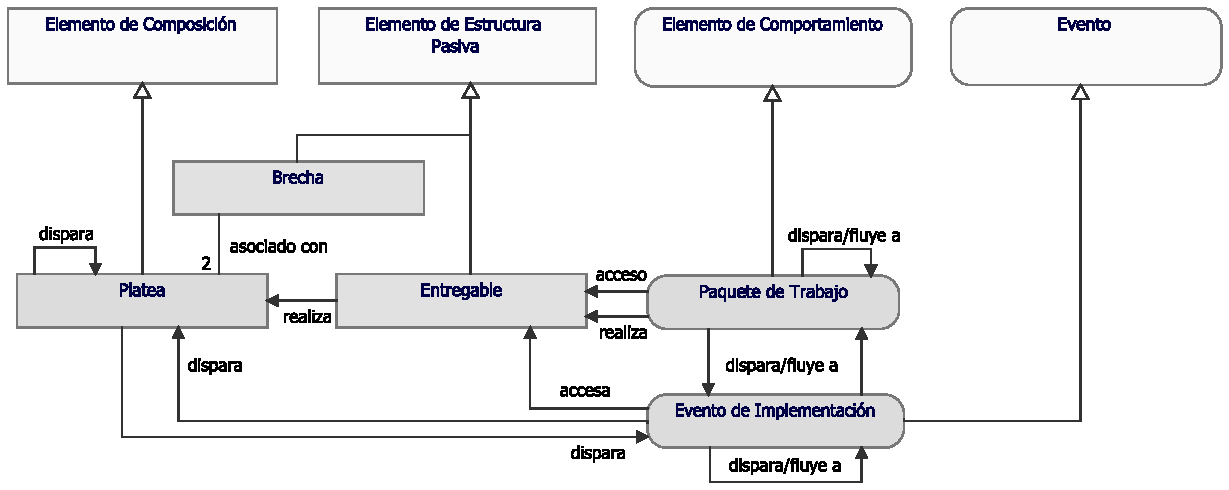
\includegraphics[width=0.9\linewidth]{imgs/meta/Proyecto}
	\caption{Metamodelo Proyecto}
	\label{fig:mProyecto}
\end{figure}

En la figura \ref{fig:mProyecto} se presenta un panorama general de los elementos de aplicación y migración y sus relaciones.\\

Los elementos de implementación y migración utilizan las relaciones estándar de ArchiMate. Se puede asignar una función comercial a un paquete de trabajo.
Una meseta está ligada a una arquitectura que es válida durante un cierto período de tiempo. Para indicar qué partes de la arquitectura pertenecen a una cierta meseta, una meseta puede agregar o componer cualquiera de los conceptos del lenguaje central de ArchiMate.\\

En sentido estricto, las relaciones entre los elementos de implementación y migración y los elementos de motivación son relaciones indirectas; por ejemplo, un entregable realiza un requerimiento o una meta a través de la realización de un elemento central de ArchiMate (por ejemplo, un componente de aplicación, un proceso de negocios o un servicio). Sin embargo, sigue siendo útil hacer explícitas esas relaciones, para mostrar directamente que un entregable es necesario para realizar ciertos requisitos y objetivos.\\

Además, los objetivos, resultados, capacidades y requisitos pueden asociarse con una cierta meseta; por ejemplo, ciertos requisitos pueden ser sólo aplicables a la Arquitectura de destino, mientras que otros pueden aplicarse a una cierta Arquitectura de transición.\\

Del mismo modo, las mesetas pueden utilizarse para la planificación basada en la capacidad. Esto puede modelarse mediante las relaciones de agregación o composición. Los objetivos, resultados, capacidades y requerimientos pueden ser agregados o compuestos en mesetas. Los requisitos y capacidades pueden realizarse por medio de los resultados. Dado que los resultados y las metas se realizan por medio de las capacidades y los requisitos, también pueden realizarse indirectamente por medio de los productos.

\newpage
\chapter{Proyecto}
\section{Introduccion}
La capa de Proyecto (Implementación y Despliegue) esta compuesta de los siguientes elementos:

\begin{itemize}
	\item Un paquete de trabajo representa una serie de acciones identificadas y diseñadas para lograr resultados específicos dentro de las limitaciones de tiempo y recursos especificadas.
	\item Un entregable representa un resultado definido con precisión de un paquete de trabajo.
	\item Un evento de implementación es un elemento de comportamiento que denota un cambio de estado relacionado con la implementación o la migración.
	\item Una meseta representa un estado relativamente estable de la arquitectura que existe durante un período de tiempo limitado.
	\item Una brecha representa una declaración de la diferencia entre dos p
\end{itemize}

Una brecha se asocia con los conceptos centrales que son exclusivos de una de las mesetas unidas por la brecha; es decir, los conceptos centrales que constituyen la diferencia entre estas mesetas. Un entregable puede realizar, entre otros, la implementación de una arquitectura o una parte de una arquitectura. Por lo tanto, cualquiera de los conceptos del lenguaje central de ArchiMate puede estar vinculado a un entregable por medio de una relación de realización.\\

Como la mayoría de los conceptos del lenguaje central, un elemento compuesto puede ser un paquete de trabajo agregado o un entregable. También pueden definirse relaciones más débiles. Por ejemplo, la relación de asociación puede utilizarse para mostrar que partes de la arquitectura se ven afectadas de alguna manera por determinados paquetes de trabajo.

%\newpage

\section{Metamodelo}
\begin{figure}[h!]
	\centering
	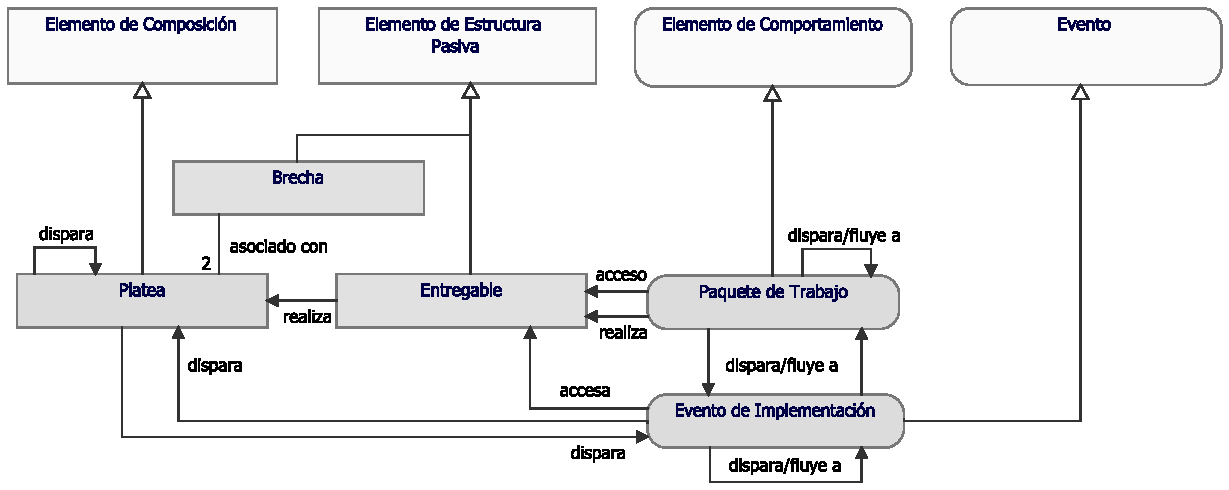
\includegraphics[width=0.9\linewidth]{imgs/meta/Proyecto}
	\caption{Metamodelo Proyecto}
	\label{fig:mProyecto}
\end{figure}

En la figura \ref{fig:mProyecto} se presenta un panorama general de los elementos de aplicación y migración y sus relaciones.\\

Los elementos de implementación y migración utilizan las relaciones estándar de ArchiMate. Se puede asignar una función comercial a un paquete de trabajo.
Una meseta está ligada a una arquitectura que es válida durante un cierto período de tiempo. Para indicar qué partes de la arquitectura pertenecen a una cierta meseta, una meseta puede agregar o componer cualquiera de los conceptos del lenguaje central de ArchiMate.\\

En sentido estricto, las relaciones entre los elementos de implementación y migración y los elementos de motivación son relaciones indirectas; por ejemplo, un entregable realiza un requerimiento o una meta a través de la realización de un elemento central de ArchiMate (por ejemplo, un componente de aplicación, un proceso de negocios o un servicio). Sin embargo, sigue siendo útil hacer explícitas esas relaciones, para mostrar directamente que un entregable es necesario para realizar ciertos requisitos y objetivos.\\

Además, los objetivos, resultados, capacidades y requisitos pueden asociarse con una cierta meseta; por ejemplo, ciertos requisitos pueden ser sólo aplicables a la Arquitectura de destino, mientras que otros pueden aplicarse a una cierta Arquitectura de transición.\\

Del mismo modo, las mesetas pueden utilizarse para la planificación basada en la capacidad. Esto puede modelarse mediante las relaciones de agregación o composición. Los objetivos, resultados, capacidades y requerimientos pueden ser agregados o compuestos en mesetas. Los requisitos y capacidades pueden realizarse por medio de los resultados. Dado que los resultados y las metas se realizan por medio de las capacidades y los requisitos, también pueden realizarse indirectamente por medio de los productos.

\newpage
\chapter{Proyecto}
\section{Introduccion}
La capa de Proyecto (Implementación y Despliegue) esta compuesta de los siguientes elementos:

\begin{itemize}
	\item Un paquete de trabajo representa una serie de acciones identificadas y diseñadas para lograr resultados específicos dentro de las limitaciones de tiempo y recursos especificadas.
	\item Un entregable representa un resultado definido con precisión de un paquete de trabajo.
	\item Un evento de implementación es un elemento de comportamiento que denota un cambio de estado relacionado con la implementación o la migración.
	\item Una meseta representa un estado relativamente estable de la arquitectura que existe durante un período de tiempo limitado.
	\item Una brecha representa una declaración de la diferencia entre dos p
\end{itemize}

Una brecha se asocia con los conceptos centrales que son exclusivos de una de las mesetas unidas por la brecha; es decir, los conceptos centrales que constituyen la diferencia entre estas mesetas. Un entregable puede realizar, entre otros, la implementación de una arquitectura o una parte de una arquitectura. Por lo tanto, cualquiera de los conceptos del lenguaje central de ArchiMate puede estar vinculado a un entregable por medio de una relación de realización.\\

Como la mayoría de los conceptos del lenguaje central, un elemento compuesto puede ser un paquete de trabajo agregado o un entregable. También pueden definirse relaciones más débiles. Por ejemplo, la relación de asociación puede utilizarse para mostrar que partes de la arquitectura se ven afectadas de alguna manera por determinados paquetes de trabajo.

%\newpage

\section{Metamodelo}
\begin{figure}[h!]
	\centering
	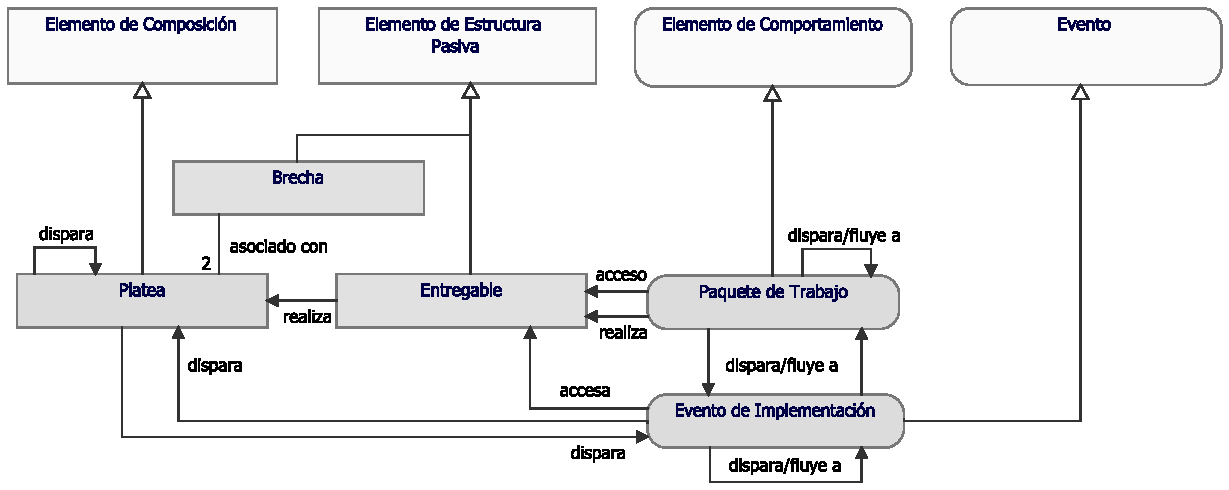
\includegraphics[width=0.9\linewidth]{imgs/meta/Proyecto}
	\caption{Metamodelo Proyecto}
	\label{fig:mProyecto}
\end{figure}

En la figura \ref{fig:mProyecto} se presenta un panorama general de los elementos de aplicación y migración y sus relaciones.\\

Los elementos de implementación y migración utilizan las relaciones estándar de ArchiMate. Se puede asignar una función comercial a un paquete de trabajo.
Una meseta está ligada a una arquitectura que es válida durante un cierto período de tiempo. Para indicar qué partes de la arquitectura pertenecen a una cierta meseta, una meseta puede agregar o componer cualquiera de los conceptos del lenguaje central de ArchiMate.\\

En sentido estricto, las relaciones entre los elementos de implementación y migración y los elementos de motivación son relaciones indirectas; por ejemplo, un entregable realiza un requerimiento o una meta a través de la realización de un elemento central de ArchiMate (por ejemplo, un componente de aplicación, un proceso de negocios o un servicio). Sin embargo, sigue siendo útil hacer explícitas esas relaciones, para mostrar directamente que un entregable es necesario para realizar ciertos requisitos y objetivos.\\

Además, los objetivos, resultados, capacidades y requisitos pueden asociarse con una cierta meseta; por ejemplo, ciertos requisitos pueden ser sólo aplicables a la Arquitectura de destino, mientras que otros pueden aplicarse a una cierta Arquitectura de transición.\\

Del mismo modo, las mesetas pueden utilizarse para la planificación basada en la capacidad. Esto puede modelarse mediante las relaciones de agregación o composición. Los objetivos, resultados, capacidades y requerimientos pueden ser agregados o compuestos en mesetas. Los requisitos y capacidades pueden realizarse por medio de los resultados. Dado que los resultados y las metas se realizan por medio de las capacidades y los requisitos, también pueden realizarse indirectamente por medio de los productos.

\newpage
\chapter{Proyecto}
\section{Introduccion}
La capa de Proyecto (Implementación y Despliegue) esta compuesta de los siguientes elementos:

\begin{itemize}
	\item Un paquete de trabajo representa una serie de acciones identificadas y diseñadas para lograr resultados específicos dentro de las limitaciones de tiempo y recursos especificadas.
	\item Un entregable representa un resultado definido con precisión de un paquete de trabajo.
	\item Un evento de implementación es un elemento de comportamiento que denota un cambio de estado relacionado con la implementación o la migración.
	\item Una meseta representa un estado relativamente estable de la arquitectura que existe durante un período de tiempo limitado.
	\item Una brecha representa una declaración de la diferencia entre dos p
\end{itemize}

Una brecha se asocia con los conceptos centrales que son exclusivos de una de las mesetas unidas por la brecha; es decir, los conceptos centrales que constituyen la diferencia entre estas mesetas. Un entregable puede realizar, entre otros, la implementación de una arquitectura o una parte de una arquitectura. Por lo tanto, cualquiera de los conceptos del lenguaje central de ArchiMate puede estar vinculado a un entregable por medio de una relación de realización.\\

Como la mayoría de los conceptos del lenguaje central, un elemento compuesto puede ser un paquete de trabajo agregado o un entregable. También pueden definirse relaciones más débiles. Por ejemplo, la relación de asociación puede utilizarse para mostrar que partes de la arquitectura se ven afectadas de alguna manera por determinados paquetes de trabajo.

%\newpage

\section{Metamodelo}
\begin{figure}[h!]
	\centering
	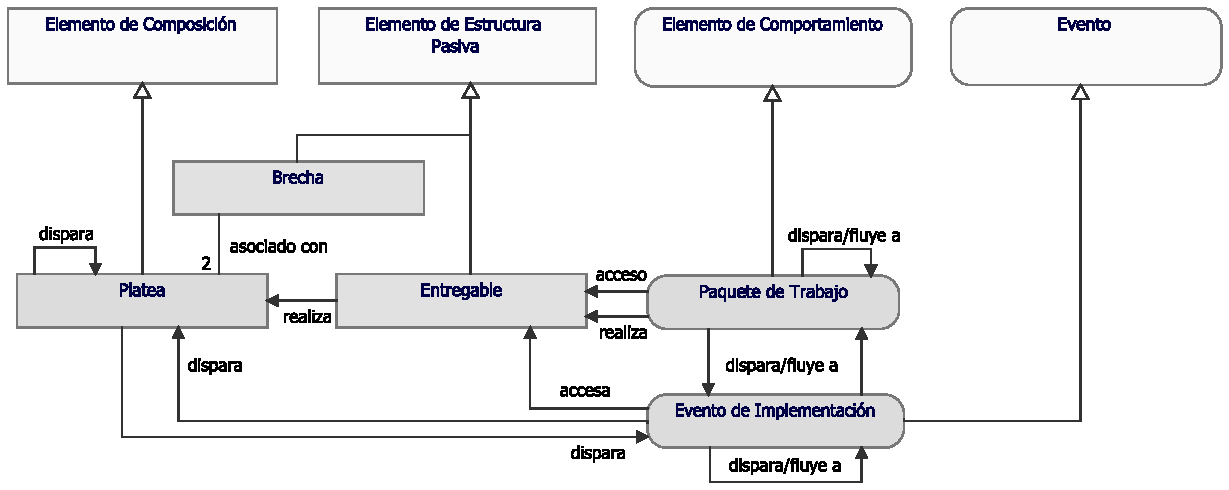
\includegraphics[width=0.9\linewidth]{imgs/meta/Proyecto}
	\caption{Metamodelo Proyecto}
	\label{fig:mProyecto}
\end{figure}

En la figura \ref{fig:mProyecto} se presenta un panorama general de los elementos de aplicación y migración y sus relaciones.\\

Los elementos de implementación y migración utilizan las relaciones estándar de ArchiMate. Se puede asignar una función comercial a un paquete de trabajo.
Una meseta está ligada a una arquitectura que es válida durante un cierto período de tiempo. Para indicar qué partes de la arquitectura pertenecen a una cierta meseta, una meseta puede agregar o componer cualquiera de los conceptos del lenguaje central de ArchiMate.\\

En sentido estricto, las relaciones entre los elementos de implementación y migración y los elementos de motivación son relaciones indirectas; por ejemplo, un entregable realiza un requerimiento o una meta a través de la realización de un elemento central de ArchiMate (por ejemplo, un componente de aplicación, un proceso de negocios o un servicio). Sin embargo, sigue siendo útil hacer explícitas esas relaciones, para mostrar directamente que un entregable es necesario para realizar ciertos requisitos y objetivos.\\

Además, los objetivos, resultados, capacidades y requisitos pueden asociarse con una cierta meseta; por ejemplo, ciertos requisitos pueden ser sólo aplicables a la Arquitectura de destino, mientras que otros pueden aplicarse a una cierta Arquitectura de transición.\\

Del mismo modo, las mesetas pueden utilizarse para la planificación basada en la capacidad. Esto puede modelarse mediante las relaciones de agregación o composición. Los objetivos, resultados, capacidades y requerimientos pueden ser agregados o compuestos en mesetas. Los requisitos y capacidades pueden realizarse por medio de los resultados. Dado que los resultados y las metas se realizan por medio de las capacidades y los requisitos, también pueden realizarse indirectamente por medio de los productos.

\newpage
\include{arquitectura/proyecto/proyecto}
\newpage
\include{arquitectura/proyecto/migracion}
\newpage
\include{arquitectura/proyecto/implementacion}
\newpage
\section{Punto de Vista de Migración}
\newpage
\section{Punto de Vista de Implmenetación y Migración}
\newpage
\section{Punto de Vista de Migración}
\newpage
\section{Punto de Vista de Implmenetación y Migración}
\newpage
\section{Punto de Vista de Migración}
\newpage
\section{Punto de Vista de Implmenetación y Migración}